\chapter{Nodal Analysis}

\section{Basic Idea}
A circuit with $b$ branches has $2b$ unknowns since there are $b$ voltages and $b$ currents. Hence, $2b$ linear independent equations are required to solve the circuit. If the circuit has $n$ nodes and $b$ branches, it has
\begin{itemize}
 \item Kirchoff's current law (KCL) equations
 \item Kirchoff's voltage law (KVL) equations
 \item Characteristic equations (Ohm's Law in a broad sense.)
\end{itemize}  
There are only $n-1$ KCLs since the nth equation is a linear combination of the remaining $n-1$. At the same time, it can be demonstrated that if we can imagine a very high number of
closed paths in the network only $b-n+1$ are able to provide independent KVLs. Finally there are $b$ characteristic equations, describing the behavior of the branch, making a total of $2b$ linear independent equations.

To prove the number of independent KVLs equations, let us consider a generic electrical circuit. Let us now substitute the circuit with one oriented graph i.e. with a diagram composed of oriented arcs where each arc represents one of the branches of the original circuit.
With this substitution we can focus simply on the topology disregarding the characteristics of the specific branch. In effect our conclusion regarding the KVL must be valid for every network no matter the branches involved and then it makes sense to focus
only on the connections.

\begin{figure}[ht]
	\centering
	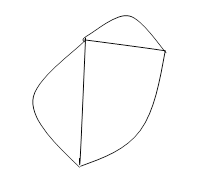
\includegraphics[scale=0.6]{img/graph_representation_1.png} 
	\caption{Graph representing the topology of an electrical circuit}
	\label{fig:graph_rep_1}
\end{figure}

Let us now orient the arc, exactly as we assume to assume a direction for the measurement of the current and let us also number the arcs.

\begin{figure}[ht]
	\centering
	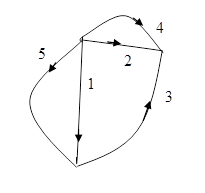
\includegraphics[scale=0.6]{img/graph_representation_2.png} 
	\caption{Oriented graph representing the topology of an electrical circuit}
	\label{fig:graph_rep_2}
\end{figure}

Let us now define a so called tree for this graph. A tree is given by a subset of arcs that connects all the nodes but do not create any closed path.

\begin{figure}[ht]
	\centering
	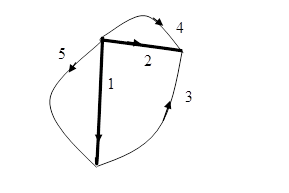
\includegraphics[scale=0.6]{img/graph_representation_3.png} 
	\caption{Selecting a tree of the graph}
	\label{fig:graph_rep_3}
\end{figure}

It is pretty easy to understand that to connect $n$ nodes without creating a closed path we are going to need $n-1$ arcs. As result $b-n+1$ arcs are not included in the tree (this is actually called co-tree).

For this network for example we have:
\begin{align}
\begin{split}
	b &= 5 \\
	n &= 3
\end{split}
\end{align}

So the tree includes 2 branches and the co-tree includes 3 branches.

\section{Basic Steps}
The nodal analysis method reduces the number of equations that need to be solved simultaneously. $n-1$ voltage variables are defined and solved, writing $n-1$ KCL based equations. 
A circuit can be solved using Nodal Analysis, by observing the following steps:

\begin{itemize}
\item Step 1: Select a reference node (mathematical ground) and number the remaining $n-1$ nodes, that are the independent voltage variables
\item Step 2: Represent every branch current $i$ as a function of node voltage variables $e$ with the general expression $i_k = g(e)$
\item Step 3: Write $n-1$ KCL based equations in terms of node voltage variable. The resulting equations can be written in matrix form and has to be solved for $e$.
\begin{equation} \label{eq:nodalAnalysis}
G_{n-1}e_{n-1} =  A_{n-1}
\end{equation}
\end{itemize}

\section{Matrix Stamp Concept}
The matrix stamp concept is an approach to construct the matrix equation \ref{eq:nodalAnalysis}. Each element of the circuit will stamp the matrix equation in certain position.

\subsection{Resistor}
A resistor R between the nodes j and k will stamp the conductance matrix $G$ in the positions j,j and k,k with the value $\frac{1}{R} $ and in the positions j,k and k,j with the value $\frac{-1}{R} $.

\begin{align}
\begin{split}
&
\begin{matrix}
& \cdots & j & \quad k & \cdots
\end{matrix}\\[-5pt]
G \quad = \quad
\begin{matrix}
\vdots\\[6pt]
j\\[6pt]
k\\[6pt]
\vdots\\
\end{matrix}
&
\begin{bmatrix}
	\quad & \quad &  \\[6pt]
	\quad & \dfrac{1}{R} & \dfrac{-1}{R} & \quad  \\[6pt]
	\quad & \dfrac{-1}{R} & \dfrac{1}{R} & \quad \\[6pt]
	\quad &  & 
\end{bmatrix}
\end{split}
\end{align}

\begin{figure}[h]
	\centering
	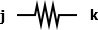
\includegraphics[scale=0.6]{img/Resistor.png}
	\caption{Resistor between nodes j and k}
	\label{fig:Resistor}
\end{figure}

\subsection{Current Source}
A current source of $I$ Ampere entering node j and leaving node k will stamp the vector $A$ at line j with $I$ and at line k with $-I$.

\begin{equation}
A \quad  = \quad
\begin{matrix}
\vdots\\
j\\[6pt]
k\\
\vdots
\end{matrix}
\begin{bmatrix}
	\\
	I \\[6pt]
	-I \\
	 \\
\end{bmatrix}
\end{equation}

\subsection{Voltage Source}
An ideal voltage source cannot be included in nodal analysis. In this case, the modified nodal analysis approach is used. The voltage source is represented, by adding a new equation to the problem and adding the current trough the voltage source $i_{jk}$ as unknown. 
For a voltage source with positive terminal connected to node j and negative terminal connected to node k. The added equation is the following:
\begin{equation}
e_j - e_k = V
\end{equation}
Moreover, the current trough the voltage source is added in the equation of node j and subtracted in the equation of node k.
The conductance matrix $G$ and the vector $A$ are stamped as following.

\begin{align}
	& \begin{matrix}
	& \cdots & j & \cdots & k & \cdots & \cdots\\[-6pt]
	\end{matrix}\\
	\begin{matrix}
	\vdots\\
	j\\
	\vdots\\
	k\\
	\vdots\\
	\vdots\\
	\end{matrix}
	& \begin{bmatrix}
	\quad & \quad & \quad & \quad & \quad & 0\\[6pt]
	& & & & & 1\\[6pt]
	& & & & & 0\\[6pt]
	& & & & & -1\\[6pt]
	& & & & & 0\\[6pt]
	0 & 1 & 0 & -1 & 0 & 0\\
	\end{bmatrix}
	\begin{bmatrix}
	\vdots \\
	e_j\\[6pt]
	\vdots \\
	e_k\\[6pt]
	\vdots\\
	i_{jk}\\
	\end{bmatrix}
	=
	\begin{bmatrix}
	\\[6pt]
	\\[6pt]
	\\[6pt]
	\\[6pt]
	\\[6pt]
	V\\
	\end{bmatrix}	
\end{align}

\subsection{Other components}
Components such as capacitor, inductor and real voltage source can be represented by equivalent circuits, composed by current source and resistance. In this way, the matrix stamp of these components is made by stamping an equivalent current source and resistance on the respective matrices. 
This approach is detailed in "Simulator Models".

 
\section{Resistive Companion Method}

\subsection{Capacitor and Inductor}
These components need some kind of memory since their behavior is dependent on the past.

\begin{equation}
        v_L(t) = L \frac{di_L(t)}{dt} \rightarrow i_L(t) = i_L(t-\delta t)+\frac{1}{L} \int_{t-\delta t}^t v_L(\tau)d\tau
\end{equation}

\begin{equation}
        i_C(t) = L \frac{dv_C(t)}{dt} \rightarrow v_C(t) = v_C(t-\delta t)+\frac{1}{C} \int_{t-\delta t}^t i_C(\tau)d\tau
\end{equation}

